\documentclass[main]{subfiles}
\begin{document}
%@@@@@@@@@@@@@@@@@@@@@@@@@@@@@@
% summarizes lecture 2
% author: David Bontrager and Benjamin Ellenberger

\section{MOSFETs}
Metal-Oxide-Semiconductor Field-Effect Transistor, built using MOS and a p-n junction diode.
\subsection{n- and p-FETs, in an n–well Process}

A MOSFET is a type of transistor that consists of  two p-n junctions, called either native transistors or well transistors depending on the composition of the p-type and n-type substrates. Native transistors sit in the substrate wafer doping type (or in wells of the same type as the substrate). The native transistor contains of two n-doped terminals and the gate. It is called native, because it is directly located in the p substrate. The pn junction is thereby given between the substrate and the n-doped terminals. Native transistors have n-type sources and drains and form an n-type channel in the p-substrate. \\ Well transistors sit in wells of the opposite type as the substrate. The well transistor in the p substrate needs an additional terminal, because its terminals are p-doped. An n-well chip for instance sits in an n-well and the substrate is p-type.  The well has p-type sources and drains and forms a p-channel in the n-well.
\begin{figure}[H]
\centering
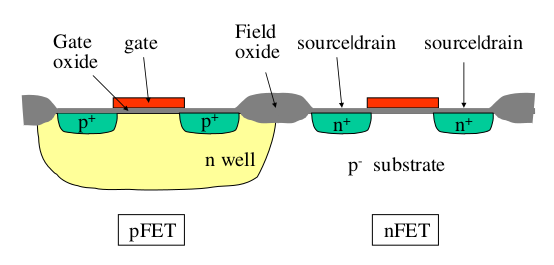
\includegraphics[width=0.6\linewidth]{figs/Field-effect-transistors.png}
\caption{Cross-section of a complementary pair of Field-Effect Transistor (FET)}
\label{field-effect transistor}
\end{figure}

FETs are generally symmetrical and the names of the terminals are defined by how it is connected. In an n-FET, electrons are transported through an electron channel. In a p-FET, electron holes are transported through an electron hole channel. Thus, the source terminal of the transistor is defined as the source of the majority carriers, which are electrons or electron holes respectively.\\

\begin{figure}[H]
  \centering
  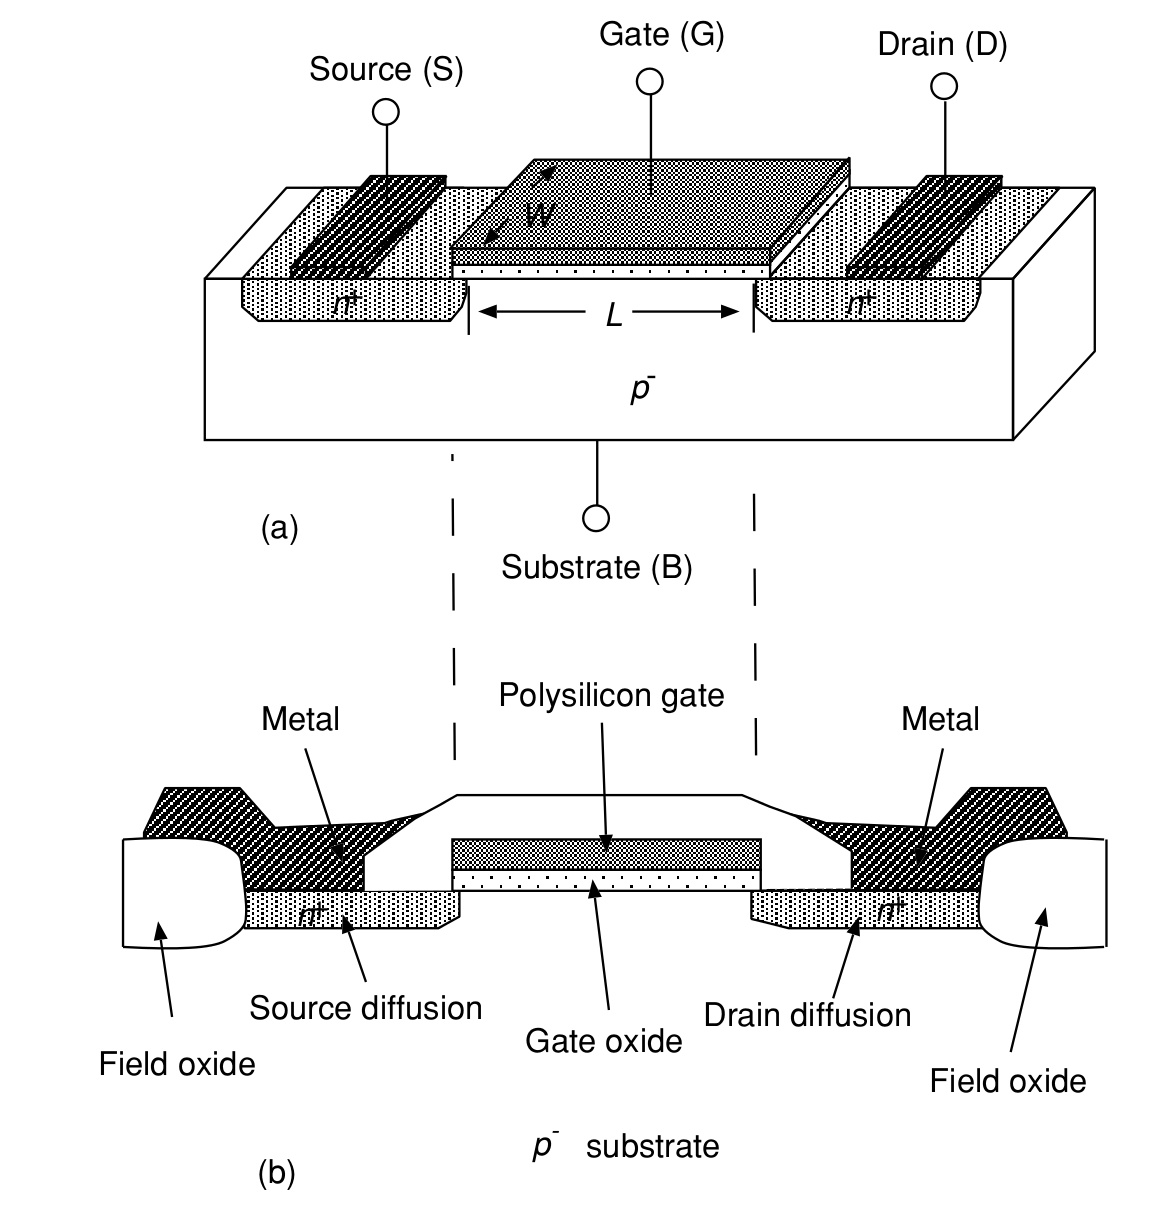
\includegraphics[scale=0.8]{figs/MOSFET_Structure.jpg}
  \caption{Structure of an n-type MOSFET in a p-body. The MOSFET has four terminals; the drain (D), the source (S), the gate (G), and the bulk (B). (a) Pictorial view of the MOSFET. (b) A more realistic picture of a cross-section of a fabricated MOSFET. Note that the gate oxide is much thinner than the field oxide. \cite{book:VLSI}}
  \label{fig:MOSFET_Structure}
\end{figure}\bigskip

\bigskip\subsection{MOS Transistor Terminals}
We can view the transistor as having four terminals:
\begin{enumerate}
\item Gate (G)
\item Source (S)
\item Drain (D)
\item Bulk (B)
\end{enumerate}

\bigskip\subsection{MOS Transistor Types}
\subsubsection{n-type}
    Because the n+ source and drain regions can supply a lot of electrons to the channel, this device is called an n-channel MOSFET (nFET,n-type MOSFET, NMOS) \cite{book:VLSI}
\subsubsection{p-type}
   In p-channel MOSFET (pFET,p-type MOSFET, PMOS) , the charge in the channel is carried by holes supplied from the source and drain regions.
    
\bigskip\subsection{MOS Transistor in Substrate}
Most CMOS processes use a p-type starting substrate.  The nFETs rest in the common $p^-$ substrate, and the pFETs rest in
n-wells within the substrate as shown in Fig. \ref{fig:MOSFET_Physical_Structure}

\begin{figure}[htbp]
  \centering
  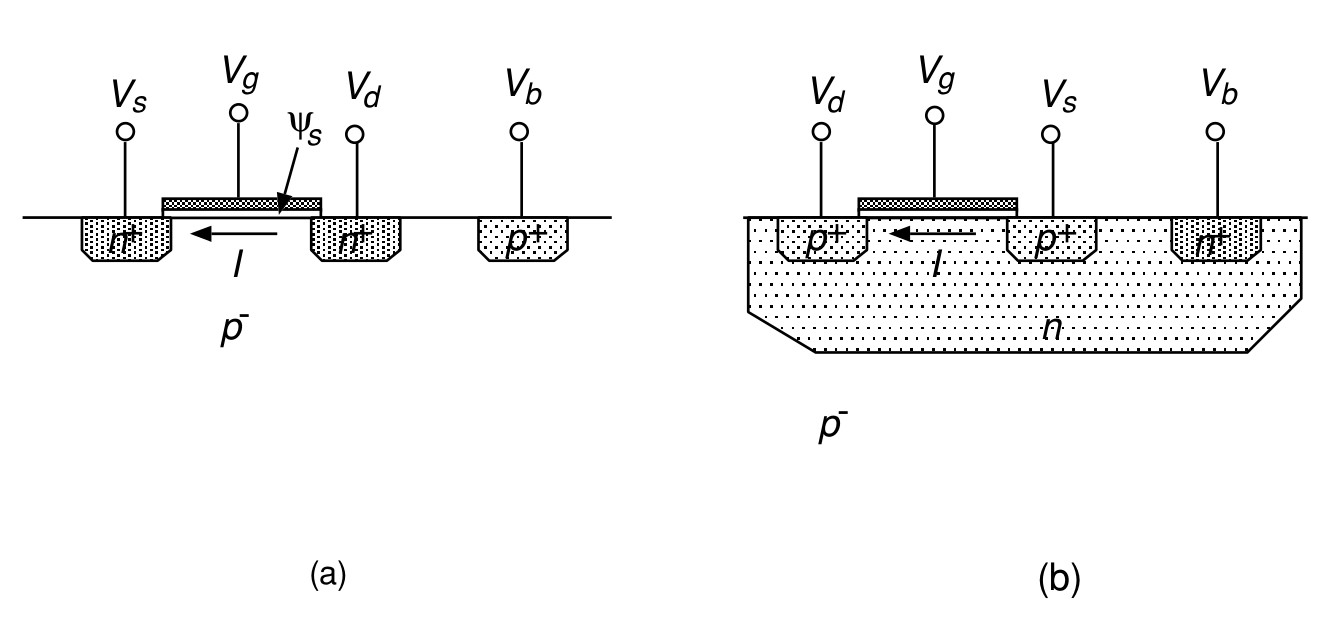
\includegraphics[scale=0.8]{figs/MOSFET_Physical_structure.jpg}
  \caption{Physical structure of (a) an nFET and (b) a pFET in a common $p^-$ substrate. The pFET rests in a n-well within the substrate. \cite{book:VLSI}}
  \label{fig:MOSFET_Physical_Structure}
\end{figure}

\subsection{Operation mode of the transistors}

A transistor can be operated in several modes. These modes have different features and different equations apply for the current between source and drain. Up to now, the subthreshold mode and the saturation mode are of importance:

\paragraph{Subthreshold}
For the n-FET in subthreshold mode, the following equation applies for the current between drain and source:
\begin{equation}
I_{DS,n,sub} = I_0e^{\kappa\frac{V_g}{U_T}}(e^{-\frac{V_s}{U_T}}-e^{-\frac{V_d}{U_T}})
\label{eq:nFETsub}
\end{equation}
This equation applies since the substrate is directly connected to ground and all voltages are measured in respect to bulk.
\\
For the p-FET in subthreshold mode, the following equation applies for the current between source and drain:
\begin{align}
I_{SD,p,sub} &= I_0e^{-\kappa\frac{V_g}{U_T}}(e^{\frac{V_s}{U_T}}-e^{\frac{V_d}{U_T}})\\
	&=I_0e^{-\kappa\frac{V_g-V_w}{U_T}}(e^{\frac{V_s-V_w}{U_T}}-e^{\frac{V_d-V_w}{U_T}})
\label{eq:pFETsub}
\end{align}
The p-FET is built in an n-well, thus the second equation shows the measured voltages with respect to the well.\\\\


\paragraph{Saturation mode}
For the n-FET in saturation mode, the following equation applies for the current between drain and source:
\begin{equation}
I_{DS,n,sat} = I_0e^{\frac{\kappa V_g-V_s}{U_T}}
\label{eq:nFETsat}
\end{equation}
For the p-FET in saturation mode, the equation again is corrected by the reference voltage at the well:
\begin{equation}
I_{SD,p,sat} = I_0e^{\frac{\kappa V_g-V_s+(1-\kappa)V_w}{U_T}}
\label{pFETsat}
\end{equation}

\subsection{Biasing}

In an n-FET, the drain terminal has the higher voltage than the source. In a p-FET, the source terminal has the higher voltage than the drain. When we compare it to the reference voltage, it can be stated that in an n-FET, all voltages need to be larger than ground, and in a p-FET, all voltages need to be smaller than $V_{dd}$.\\

For the n-FET holds:
\begin{equation}
0\unit{V} - 0\unit{V} < V_s - 0\unit{V} < V_d - 0\unit{V}
\label{eq:nFETbias}
\end{equation}

For the p-FET holds:
\begin{equation}
V_{dd} - V_{dd} > V_s - V_{dd} > V_d - V_{dd}
\label{eq:pFETbias}
\end{equation}

\subsection{The meaning of $\kappa$}
To understand the meaning of $\kappa$, we look at a constant channel current and a saturated transistor.

For the n-FET holds:
\begin{equation}
V_s = \kappa V_g - U_T(\mathrm{ln}(I_{DS,n,sat})-\mathrm{ln}(I_0))
\label{eq:nFETv_s}
\end{equation}

For the p-FET holds:
\begin{equation}
V_s = \kappa (V_g - V_w) - U_T(\mathrm{ln}(I_{DS,n,sat})-\mathrm{ln}(I_0)) + V_w
\label{eq:pFETv_s}
\end{equation}

The slope in both equations is the so called $\kappa$:
\begin{equation}
\frac{\partial V_s}{\partial V_g} = \kappa
\end{equation}

\subsection{MOS Transistor Biasing}

The location of drain and source is defined by the carrier flow\cite{book:VLSI}.
The majority carrier (either electrons or electron holes) is supplied to the channel by the source, and removed by the drain.

\begin{figure}[H]
\centering
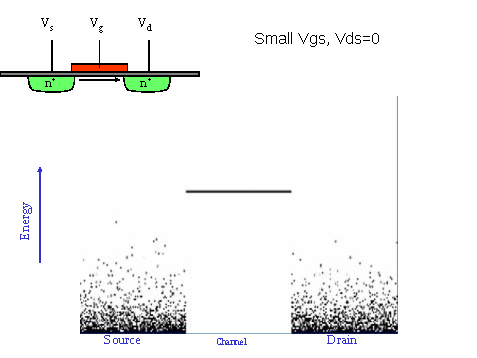
\includegraphics[scale=1]{figs/unbiased_transistor.pdf}
\caption{Unbiased transistor with energy levels of the two terminals and the channel. No net current flow.}
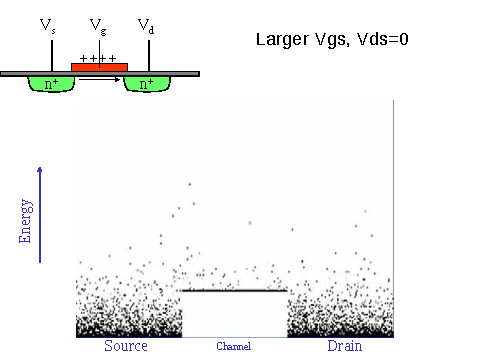
\includegraphics[scale=1]{figs/larger_vgs_transistor.pdf}
\caption{We increased $V_{gs}$ so that the barrier is lowered. Both carriers float freely but the net current is still zero.}
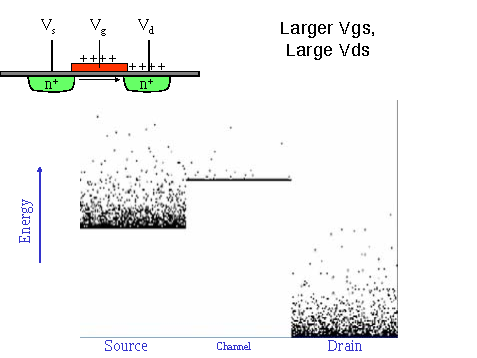
\includegraphics[scale=1]{figs/larger_vgs_vds_transistor.pdf}
\caption{We additionally increased $V_{ds}$ causing electrons to flow from source to drain.}
\end{figure}

%Ben end

\section{On capacitance, MOSFETs, and regions}
%David
We start with nomenclature. There are two basic kinds of MOSFETs\footnote{Metal-Oxide-Semiconductor [what it's made of] Field Effect Transistor [how it works]}: nFETs and pFETs. These are sometimes also called $n$-channel and $p$-channel transistors (respectively), and – in an $n$-well device – native and well transistors (respectively). The nFET has an $n$-type source and drain sitting in a $p$-type substrate, and the pFET is vice-versa.\\ \\
We have devices now – things to plug in. You tie the nFET's drain to a higher voltage than its \textsl{source} (which will \textsl{source} electrons), and the pFET is vice-versa (because it will \textsl{source} holes). ``Source'' and ``drain'' are so named because they respectively \textsl{source} and \textsl{drain} the majority mobile carrier of the given transistor type.\\ \\
You don't want current crossing the $pn$ junctions where the drain and source sit in the substrate, so we reverse bias those junctions\footnote{Put $n$ at a higher voltage than $p$}. That means we stick the nFET bulk to ground (usually hardwired on the chip), and keep $V_s, V_d > 0$. \\ \\
We know about the sub- and above threshold regions. Moving between these two regions is a function of $V_g$, specifically the voltage between the gate and the source ($V_{gs} = V_g - V_s$). Both the sub- and the above threshold regions are divided into the triode\footnote{Interesting but irrelevant: ``triode'' comes from the original thought behind the transistor as a 3-terminal diode, thus \emph{tri-}ode vs. \emph{di}-ode. The entire transistor history on Wikipedia is a really interesting read.} and saturation regimes. For both sides of the threshold, we move in and out of saturation by changing $V_{ds}$ – the drain-source voltage.\\ \\
\textsl{This is important: changing \emph{gate-source} voltage from low to high moves us from subthreshold to above threshold for \emph{any} $V_{ds} > 0$. Similarly, changing \emph{drain-source} voltage from low to high moves us from ohmic regime to saturation regime for \emph{any} $V_{gs} > 0$.} \\ \\

\subsubsection{The coupling factor $\kappa$}
Surface voltage $\psi_s$ deserves another mention. We've built a transistor, plugged it in, and biased the gate relative to the bulk\footnote{Really, we care about all voltages \emph{relative to the bulk}, but bulk is almost always at ground so it's an implicit relation}. Because of the positive gate voltage, the depletion region does not only surround the drain and source, but also extends between them. Having this channel of depletion region means that there is a built-in voltage across it\footnote{Not across it as in a \emph{drain-source} voltage, but across it as in perpendicular to the plane of the insulating oxide}. So here we have two voltages in series – one across the insulating oxide, one across the depletion region. Current isn't flowing across either of these gradients, so what does that mean? It means static, accumulated charges are hanging out on either side of the gradients. In other words: they are capacitances. The relationship between the capacitances is described by $\kappa$, which we call the \textsl{capacitive coupling ratio} from gate to channel. It describes how effectively a change in gate voltage can change the surface voltage.
The relationship between the applied potential and the surface potential is given by the coupling factor

\[\pl{\kappa = \frac{\partial \psi_s}{\partial U} = \frac{C_i}{C_i + C_d}}\]

which is the incremental capacitive divider ratio as seen from the conductor
side.


%------Transistor cross-section-------
\begin{figure}[H]
 \centering
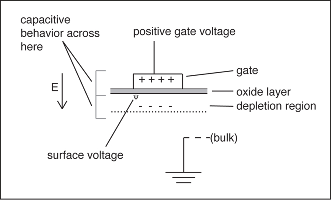
\includegraphics[width=0.8\linewidth]{figs/nme_xSection.pdf}
\caption{Cross-section of the transistor gate, oxide layer, and depletion region. When $V_{gate-bulk} > 0$, both the oxide insulator and the depletion region (channel) act as capacitors. See Figure 2.18, p.42 in the textbook for a proper version of this figure.\label{crossSectionCaps}}
\end{figure}
%-----------------------------------------------

\begin{figure}[H]
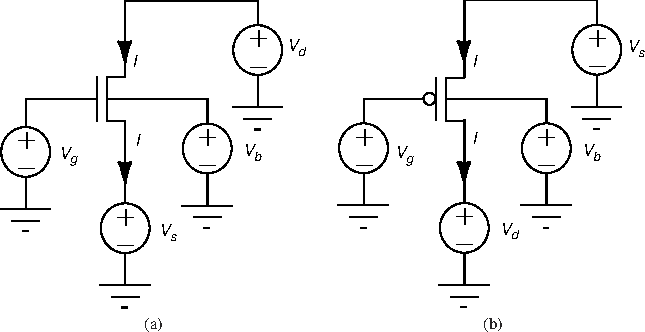
\includegraphics[width=0.8\linewidth]{figs/nFET-pFET-operation.pdf}
\caption{Biased MOSFETs showing the direction of conventional current flow. (a) For proper nFET operation, we should ensure that $V_g \geq V_b, V_s \geq V_b $ and $V_d \geq V_b$. If $V_d \geq V_s$, the channel current $I$ is positive, flowing from drain to source as shown. If $V_d \leq V_s$, then $I$ is negative and flows in the opposite direction. (b) For proper pFET operation, we should ensure that $V_g \leq V_b, V_s \leq V_b $ and $V_d \leq V_b$. If $V_d \leq V_s$, the channel current $I$ is positive, flowing from drain to source as shown. If $V_d \geq V_s$, then $I$ is negative and flows in the opposite direction.}
\end{figure}


%Joachim
\subsection{MOSFET Operation Domains}
The operation domain of an nFET is set by the relative values of the four terminals of the transistor.\\
In general, these operation domains (e.g. accumulation, depletion, weak inversion, moderate inversion, or strong inversion) are equivalent to the ones of the MIS structure.\\

\subsubsection{Subthreshold Region}
Increasing the gate voltage increases the positive charge on the gate. This
charge repels the holes in the substrate and leaves behind negatively-charged
ions, that balance out the gate charge. The MOSFET operates in the sub-
threshold regime when the positive charge on the gate is almost balanced by
the negatively-charged depletion region underneath the gate.
There is also a very thin layer of electrons beneath the gate (the inversion
layer).

We can map the regimes to a MOSFET mode:


\begin{longtable}{ |p{4cm}|p{4cm}|p{4cm}| }
\hline
\textbf{When the MOSFET is in this domain:} & \textbf{We say the MOSFET operates in:} & \textbf{Which can be further divided into (depending on $V_{gs}$:} \\ \hline
\endhead
Accumulation & Cutoff & \\ \hline
Depletion & Cutoff & \\ \hline

Weak Inversion & Subthreshold & Triode Mode \par Saturation Mode\\ \hline
 Strong Inversion & Above Threshold & Triode Mode \par Saturation Mode\\ \hline
\end{longtable}


\end{document}